\chapter{Outline}
\label{chap:out}

\section{The big picture}
\begin{figure}[tp]
  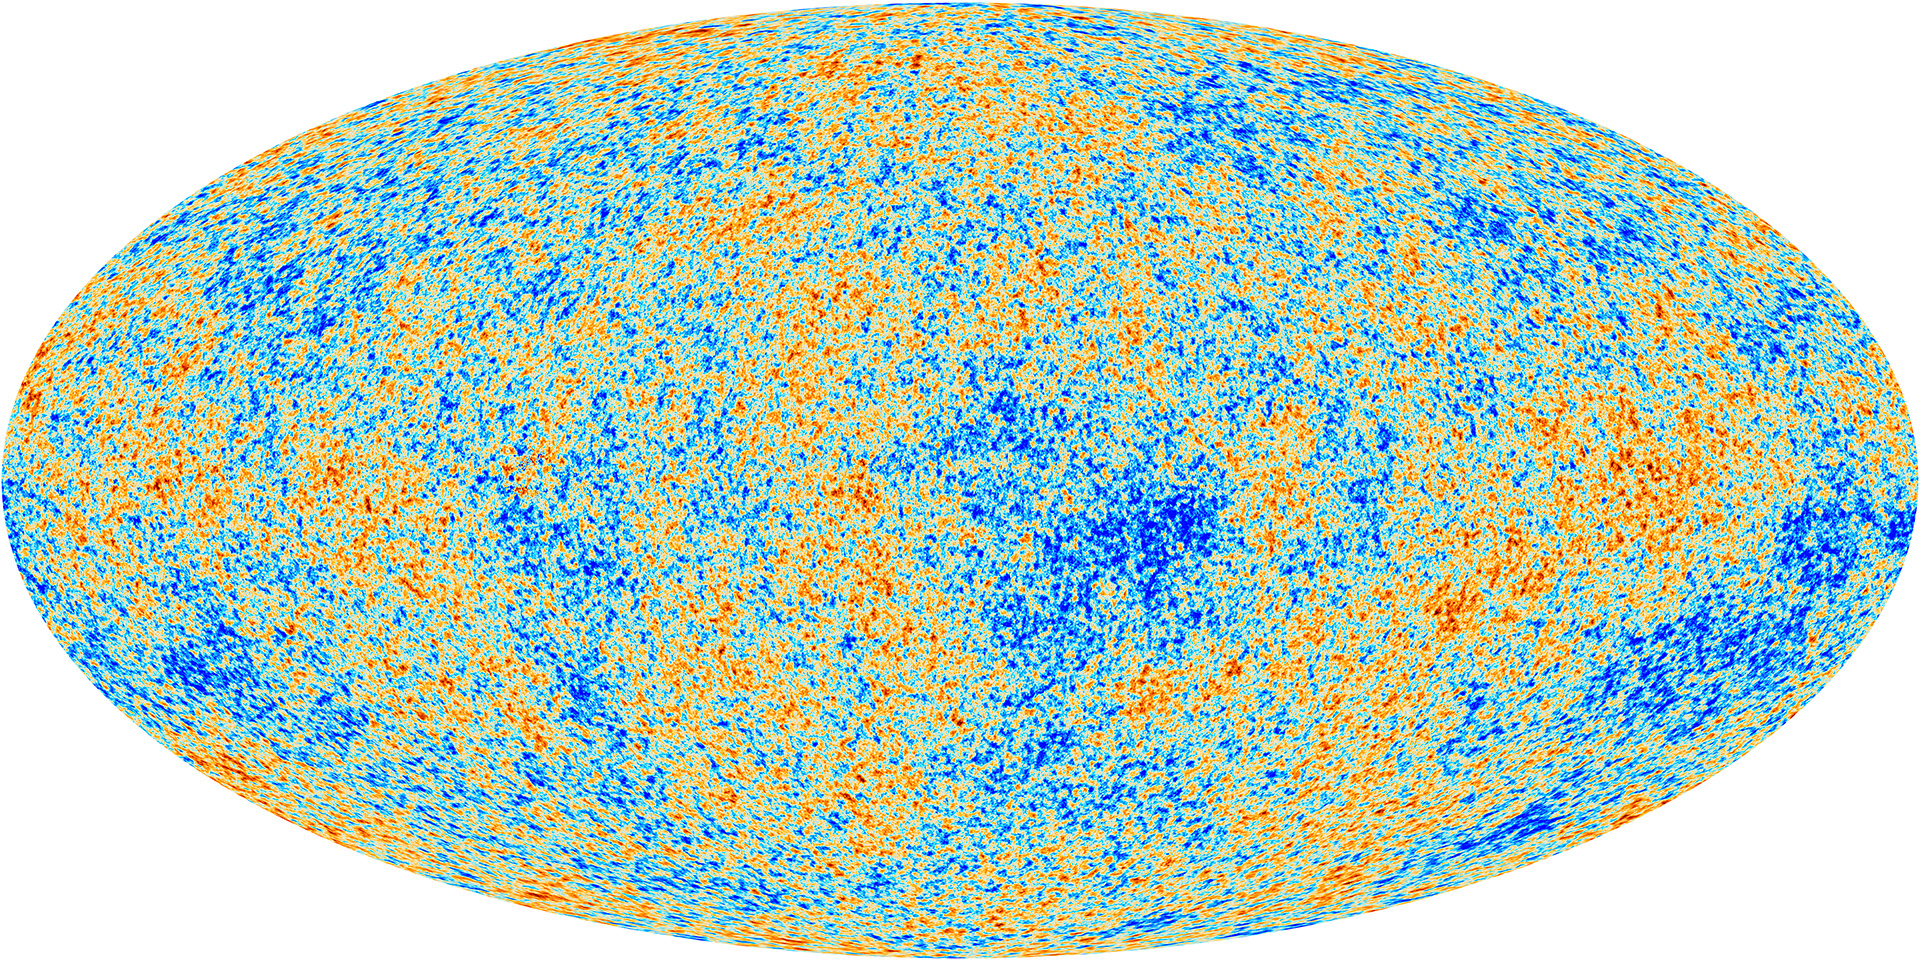
\includegraphics[width=\textwidth]{chapters/outline/figures/planck}
  \caption{Temperature distortions in the cosmic microwave background.}\label{fig:out:planck}
\end{figure}

As cosmologists, nature has been incredibly kind to us. We have been given a near crystal clear snapshot of the universe a mere 300,000 years after its birth. Images taken by the Planck satellite (Figure~\ref{fig:out:planck}) show the universe at this time, allowing us to map out the regions of higher and lower density. For cosmologists these distortions are interesting in two ways. 

First, these perturbations in density are the beginnings of the formation of stars, galaxies and galaxy clusters. If one were to wind the clock forwards from this moment, cosmic structure would be seen coalescing around the regions of higher density.

Second, these distortions tell us a great deal about physics at much earlier times. Observations from particle physics experiments allow us to confidently wind the clock backwards to mere microseconds after the big bang.
However, the expansion of the universe itself allows us to look even further back than this. We now have a wealth of observational evidence that early in its history, the universe went though an epoch of rapid accelerated expansion.  This expansion acts as a cosmic magnifying glass, allowing us to observe patterns $\sim10^{-32}$ seconds after the big bang using the universe we see today. The upshot of this is that cosmologists effectively have access to the most powerful particle accelerator imaginable, reaching energies trillions of times greater than the Large Hadron Collider. 

The canonical explanation for the early period of accelerated expansion is the theory of inflation, with quantum fields providing the necessary driving force. This thesis focusses on the initial conditions for inflation; i.e.\ what started this all off.

\section{Kinetic initial conditions}

Traditionally, cosmologists work under the assumption that at these early times the universe was in an effectively eternal inflating state, with no detectable beginning. Chapter~\ref{chap:kd} rigorously proves a result that suggests this picture may be somewhat incomplete. In fact, almost all classical universes begin at a finite time in the past. Moreover, this beginning is dominated by kinetic energy, and not inflating. This provides a novel and arguably simpler mechanism for setting the initial conditions of the universe. More importantly, I also show that this period could have produced a distinct observational signature in the primordial power spectrum of curvature perturbations.

As a member of the Planck collaboration, I began to search for evidence of this primordial signal. Chapter~\ref{chap:rec} details a model-independent reconstruction of the primordial spectrum. Whilst not conclusive, it did show tantalising hints of a signal consistent with a pre-inflationary epoch.

\section{Observations in high dimensions}
\begin{figure}[tp]
  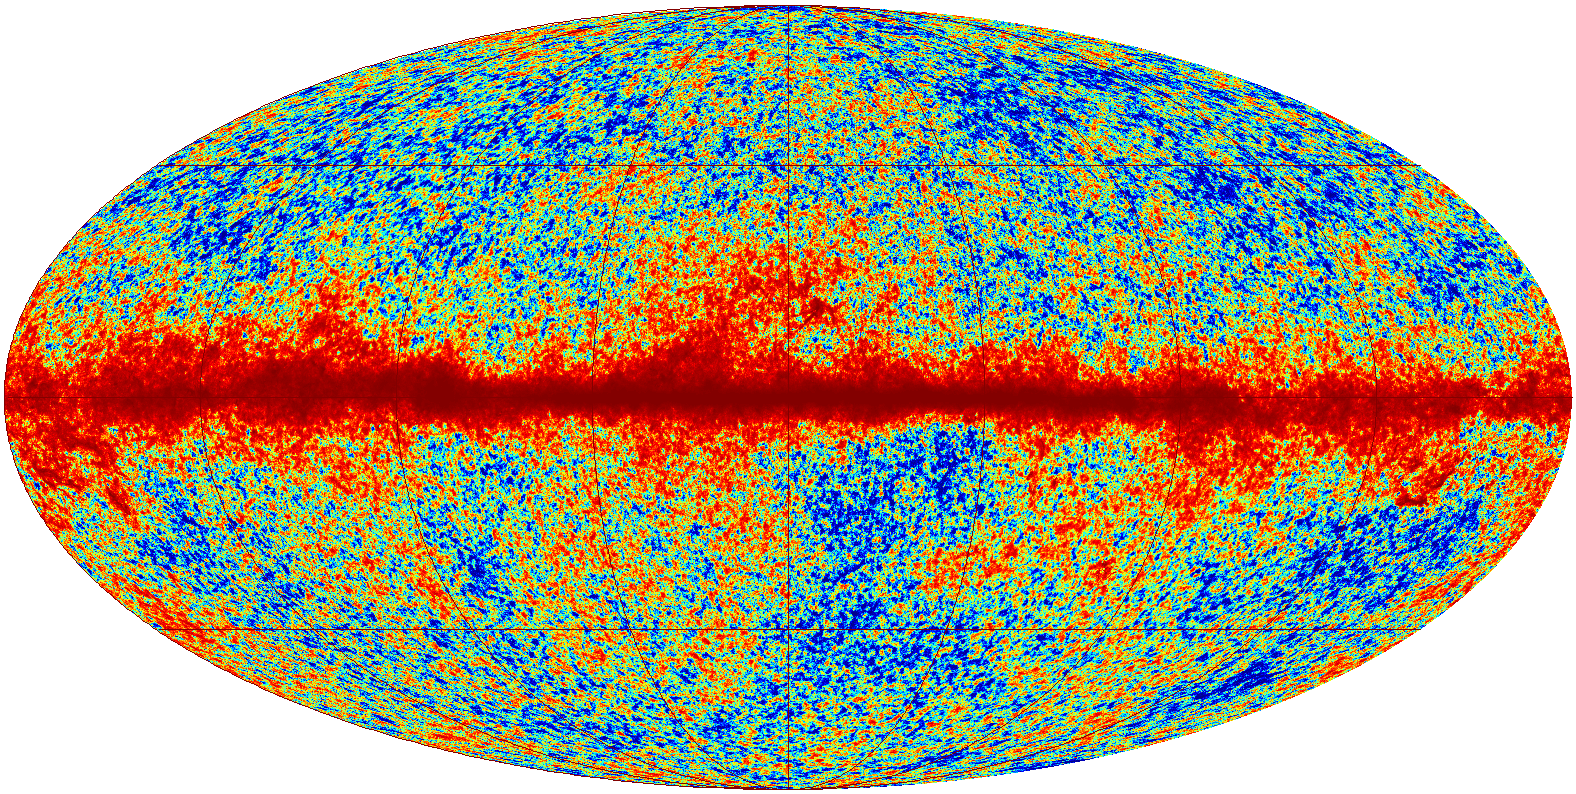
\includegraphics[width=\textwidth]{chapters/outline/figures/planck_galaxy}
  \caption{The microwave sky as seen by Planck}\label{fig:out:planck_galaxy}
\end{figure}
Planck's view of the early universe is not in fact the one shown in Figure~\ref{fig:out:planck}. The picture it actually takes is more akin to Figure~\ref{fig:out:planck_galaxy}. The most notable difference between the two is the presence of a red band in the center of the image, which are the microwaves emitted by our own Milky Way galaxy. In order to observe the microwaves generated by the beginning of the universe, we must first remove the contaminating information of the Milky Way. This requires a sophisticated model of the galaxy, with many parameters that must be simultaneously determined and quantified. 

Whilst working on Planck, it became apparent that there was an absence of Bayesian data analysis tools available for my reconstruction of the primordial signal. %@TO_DO: lengthen & make more complicated

The Cavendish Astrophysics group has a long history of developing and applying novel Bayesian statistical approaches. With this in mind, I designed and implemented a novel algorithm which was christened PolyChord (detailed in Chapter~\ref{chap:pc}). This was designed to gather information from data about complicated scientific models, whilst simultaneously calculating the probability that the model is true. PolyChord proved extremely successful in the Planck analysis, and was rapidly adopted by many members of the team as its de-facto inference tool

\section{Quantum initial conditions}
My latest work focusses on the quantum mechanical initial conditions of the early universe. A full theoretical treatment of this epoch requires a consideration of quantum fields in curved spacetime. One of the critical issues is that our basic ideas about how we talk about quantum particles are not designed to work in the context of gravity as a curved spacetime background. My latest research aims to resolve some of these issues, by re-defining the quantum mechanical notion of empty space, and building a vacuum around the renormalised stress energy tensor. I also demonstrated that in the context of the early universe this alternative viewpoint makes detectable predictions which again differ from standard theory. This is detailed in Chapter~\ref{chap:qv}.

Whilst examining this, I realised that I needed a better way of solving the equations of the early universe. I did indeed succeed in developing a novel class of extremely efficient numerical methods for solving these, which I term RKWKB approaches. RKWKB is explained Chapter~\ref{chap:RK}.

\section{Thesis versus research}

The theme of this thesis is the interplay between theory, observations and methods. Whilst the thesis is divided into two parts, in reality both halves have strongly influenced each other in a manner not necessarily consistent with the sequence of the text. Figure~\ref{fig:out:sequence} shows an approximate set of interactions between the various chapters. Whilst a thesis must be laid out sequentially, the reality is that research is often very non-linear.

\begin{figure}[tp]
  \tikzsetnextfilename{sequence}
  \tikzset{external/export next=false}

\begin{tikzpicture}[%
    node distance = 5mm,
    writing/.style={%
      text width=30mm,  % default text width
      align=center      % align in center
    },
    component/.style={%
      writing,          % writing style above
    },
    connection/.style={%
      very thick,      % very thick arrows
      >=stealth        % pretty arrow head
    }
]

  \node[component] (KD) at (0,0) {Kinetic dominance\\(Chapter~\protect\ref{chp:kd})};

  \node[below left = of KD, component] (TO)  {Theoretical observations\\(Chapter~\protect\ref{chp:kt})};

  \node[below = of KD, component] (PS) {Power spectrum reconstruction\\(Chapter~\protect\ref{chp:rec})};

  \node[right = of PS, component] (NS) {Nested sampling\\(Chapter~\protect\ref{chp:ens})};

  \node[below = of NS, component] (PC) {\PolyChord{}\\(Chapter~\protect\ref{chp:pc})};

  \node[below = of TO, component] (RE) {Quantum\\ kinetic dominance\\(Chapter~\protect\ref{chp:qv})};

  \node[below = of RE, component] (RK) {RKWKB\\(Chapter~\protect\ref{chp:RK})};

  \node[right = of RK, component] (FUT) {Constraining the kinetically dominated universe\\(Future research)};

    \draw[connection,->] (KD) -- (PS);
    \draw[connection,->] (KD) -- (TO);
    \draw[connection,->] (NS) -- (PC);
    \draw[connection,->] (PC) -- (PS);
    \draw[connection,->] (TO) -- (RE);
    \draw[connection,->] (PS) -- (RE);
    \draw[connection,->] (RE) -- (RK);
    \draw[connection,->] (RE) -- (FUT);
    \draw[connection,->] (PC) -- (FUT);
    \draw[connection,->] (RK) -- (FUT);
    \draw[connection,->] (PS) -- (FUT);

\end{tikzpicture}

  %\includegraphics[width=\textwidth]{chapters/outline/plots/sequence.tikz}
  \caption{The ``sequence'' of my research.}\label{fig:out:sequence}
\end{figure}





